\chapter*{Appendix A}
\section{Optical Phase Space}
Before analysing the different configurations of plenoptic cameras, it is important to define an useful tools that allows to better represent the light field, in order to understand and manage it better. This is the optical phase space. In the representation of light field explained in section \ref{sec:lightfield}, each ray of the light field is defined by a set of four coordinates, two spatial coordinates x and y, and the directional coordinates $\theta_x$ and $\theta_y$. Referring to figure we define momentum the quantity:
\begin{equation}
\label{eq:momentum}
\overrightarrow{p} =\dfrac{\partial \overrightarrow{q}(s)}{\partial s} 
\end{equation}
\begin{figure}[H]
	\centering
	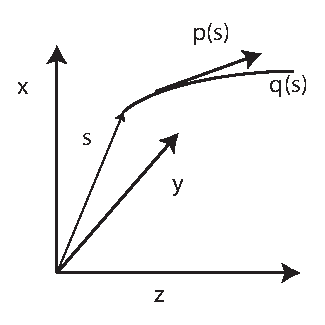
\includegraphics[width=.4\textwidth]{C:/Users/Massimo/Documents/Thesis/momentum.eps}
	\caption{\label{fig:momentum}The optical momentum correspond to the direction of the ray of light.}
\end{figure}
where $\overrightarrow{q}(s)$ is a vector describing the trajectory of a ray of light in the three dimensional space and s is the position respect the origin of the axis x,y and z. Because of the Fermat principle, considering the trajectory of the ray  $\overrightarrow{q}(s)$ as a straight line, its derivative is proportional to its angular coefficient. So we can approximate the momentum $\overrightarrow{p}$ with the direction of the ray $(\theta_x,\theta_y)$.
It is defined as a four dimensional manifold of the positions $(x,y)$ and  momentum $(p_x,p_y)$ of the rays in a certain volume \cite{wolf2004geometric} \cite{guillemin1990symplectic}. Each point in the phase space correspond to a unique ray. We will consider the phase space as a four dimensional manifold of the positions (x,y) and the directions $(\theta_x,\theta_y)$. For more details regarding the phase space refer to appendix A. 


\begin{figure}[H]
	\centering
	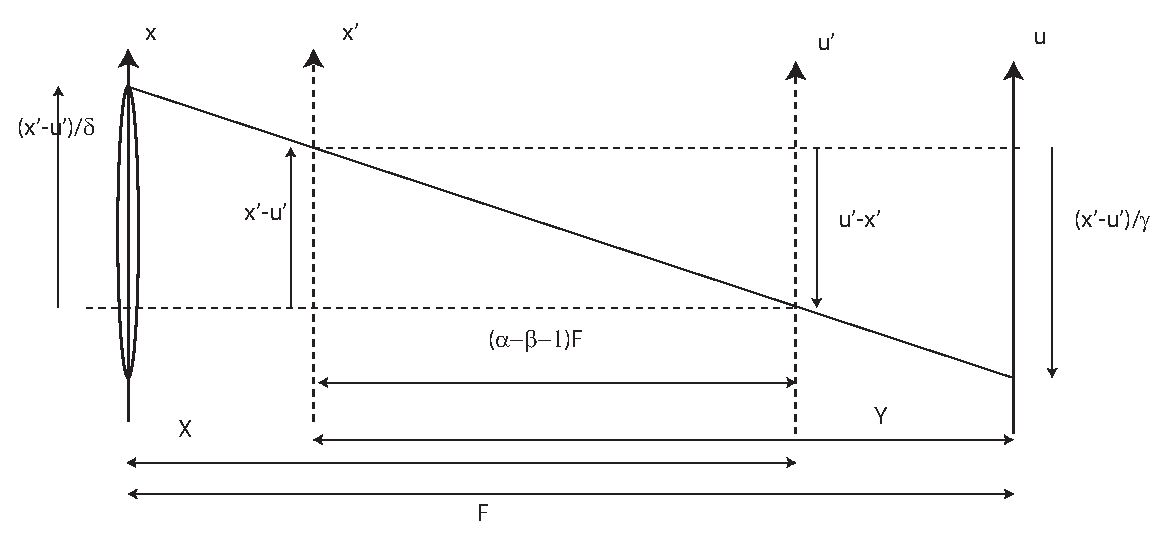
\includegraphics[width=.8\textwidth]{C:/Users/Massimo/Documents/Thesis/sinth1.eps}
	\caption{\label{fig:synthetic1} . }
\end{figure}
Referring to figure \ref{fig:synthetic1} we define
\begin{itemize}
	\item \textit{F} as the distance between the main lens and the micro lens plane.
	\item \textit{X} as the distance between the lens plane \textit{u} and the synthetic image plane \textit{u'}.
	\item \textit{Y} as the distance between the lens plane \textit{u'} and the synthetic image plane \textit{x}.
	\item $\alpha$ and $\beta$ are defined respectively as: $\alpha = X/F$ and $\beta = Y/F$
	\item the distance between the plane \textit{x'} and \textit{u'} is given by: 
	\begin{equation}
	\label{eq:dist1refoc}
	F-[F-(\beta F)]-[F-(\alpha F)]=(\alpha + \beta -1)F
	\end{equation}
	
	\item We define two further quantities for notation convenience:
	\begin{equation}
	\label{eq:refocus1}
	\left\{
	\begin{array}{l l}
	\gamma = \dfrac{\alpha +\beta -1}{\alpha} \\
	\\
	\delta = \dfrac{\alpha +\beta -1}{\beta} 
	\end{array} \right.\
	\end{equation}
\end{itemize}
Looking at figure \ref{fig:synthetic1} we note that the rays crossing the planes \textit{x'} and \textit{u'}, cross also the plane \textit{x} at the coordinates $u'+\dfrac{(x'-u')}{\delta}$ and the plane \textit{u} at the coordinate $x'+\dfrac{(u'-x')}{\gamma}$ and considering the fact that the light field is conserved during the propagation in the optical system,  we can write:
\begin{equation}
\label{eq:synthLF}
L'(x,y,u,v) = L\left(u'+\frac{(x'-u')}{\delta},v'+\frac{(y'-v')}{\delta},x'+\frac{(u'-x')}{\gamma},y'+\frac{(v'-y')}{\gamma}\right)
\end{equation}
and the intensity at the synthetic planes is given integrating the light field at the synthetic planes:
\begin{equation}
\label{eq:synthLF1}
I(x,y) =\iint L\left(x'+\frac{(x'-u')}{\delta},y'+\frac{(y'-v')}{\delta},u'+\frac{(u'-x')}{\gamma},v'+\frac{(v'-y')}{\gamma}\right)A(x',y')dudv
\end{equation}